\question[30] In this problem, we will demonstrate the basic physics of a railgun. Two very long conducting rails are held in place while a conducting rod is free to slide atop them with negligible friction but good electrical contact. The two long rails are connected to a high-voltage power supply as shown in the figure.

\begin{center}
	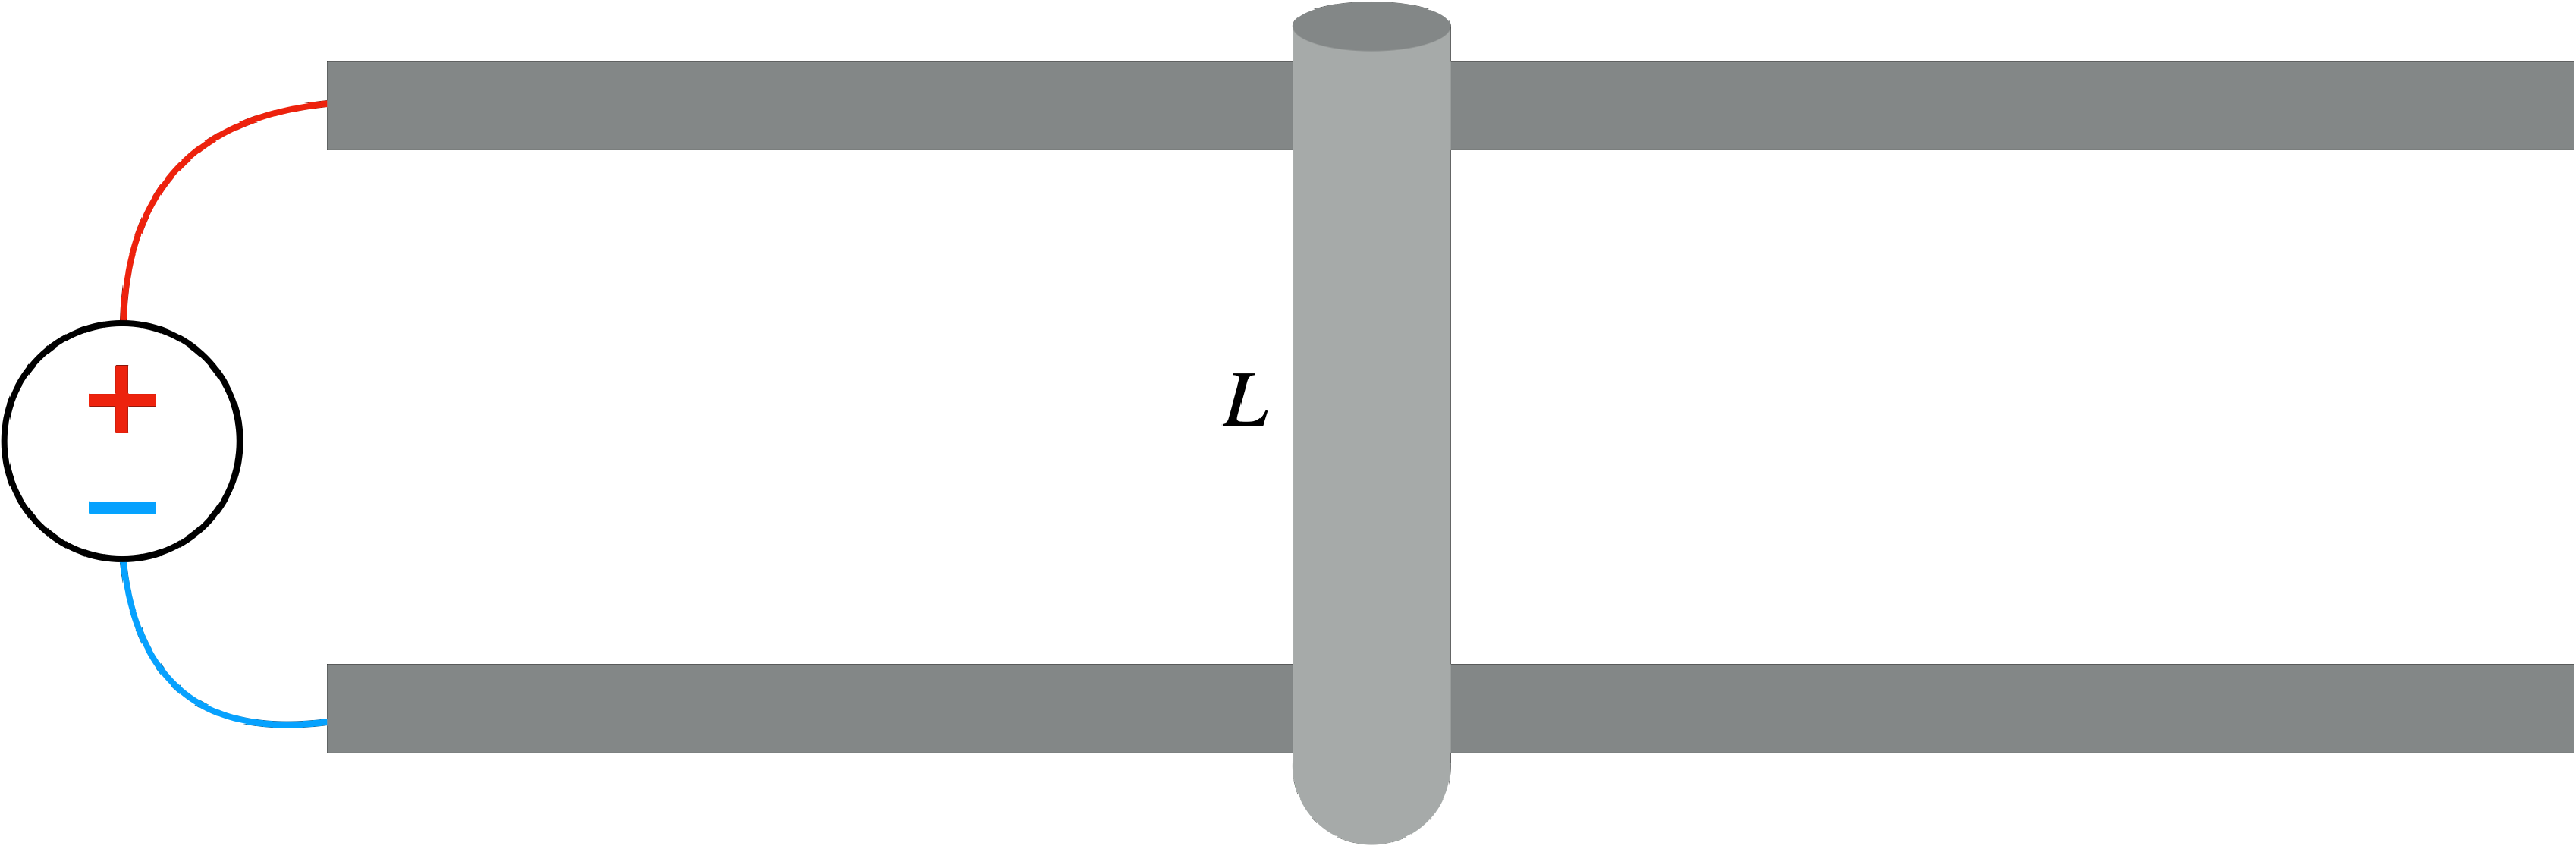
\includegraphics[width=0.5\textwidth]{rail_gun}
\end{center}

\begin{parts}
	\part Assume that the conducting rails and voltage supply have negligible resistance, and that the movable rod has a resistance of $R=1\ \Omega$. If the voltage source creates a potential difference of $\varepsilon=100,000$ V, what is the current through the circuit?
	\vspace{2cm}
	\part This current will create a magnetic field. Make the assumption that the two conducting rails are extremely long, and that they are the only wires which contribute to the magnetic field. The two conducting rails are a distance $L=0.5$ m apart. What is the magnetic field due to the two long conducting rails at the midpoint between them? Be sure to specify both magnitude and direction.
	\vspace{3cm}
	\part Now, make the assumption that the magnetic field you found in the previous part is uniform and fills the entire region (this is not actually true, but will help give us a \textit{basic} idea of how the railgun works).
	
	This magnetic field exerts a force on the current-carrying movable rod which causes it to accelerate. What is the initial acceleration of the rod if it has a mass of 10 kg? (The length of the rod is $L=0.5$ m).
	
	\vspace{3cm}
	\part As the sliding rod picks up speed $v$, an induced motional emf is generated. What is the direction of the induced motional emf (does it tend to drive current clockwise or counter-clockwise)?
	\vspace{1cm}
	\part Assuming that the magnetic field remains constant, at what speed $v$ will the motional emf equal the voltage of the voltage supply ($100,000$ V)?
\end{parts}